\section{Traveaux de modélisations} 

\subsection{Diagrammes d'activités}

\begin{figure}[h!]
\begin{center}
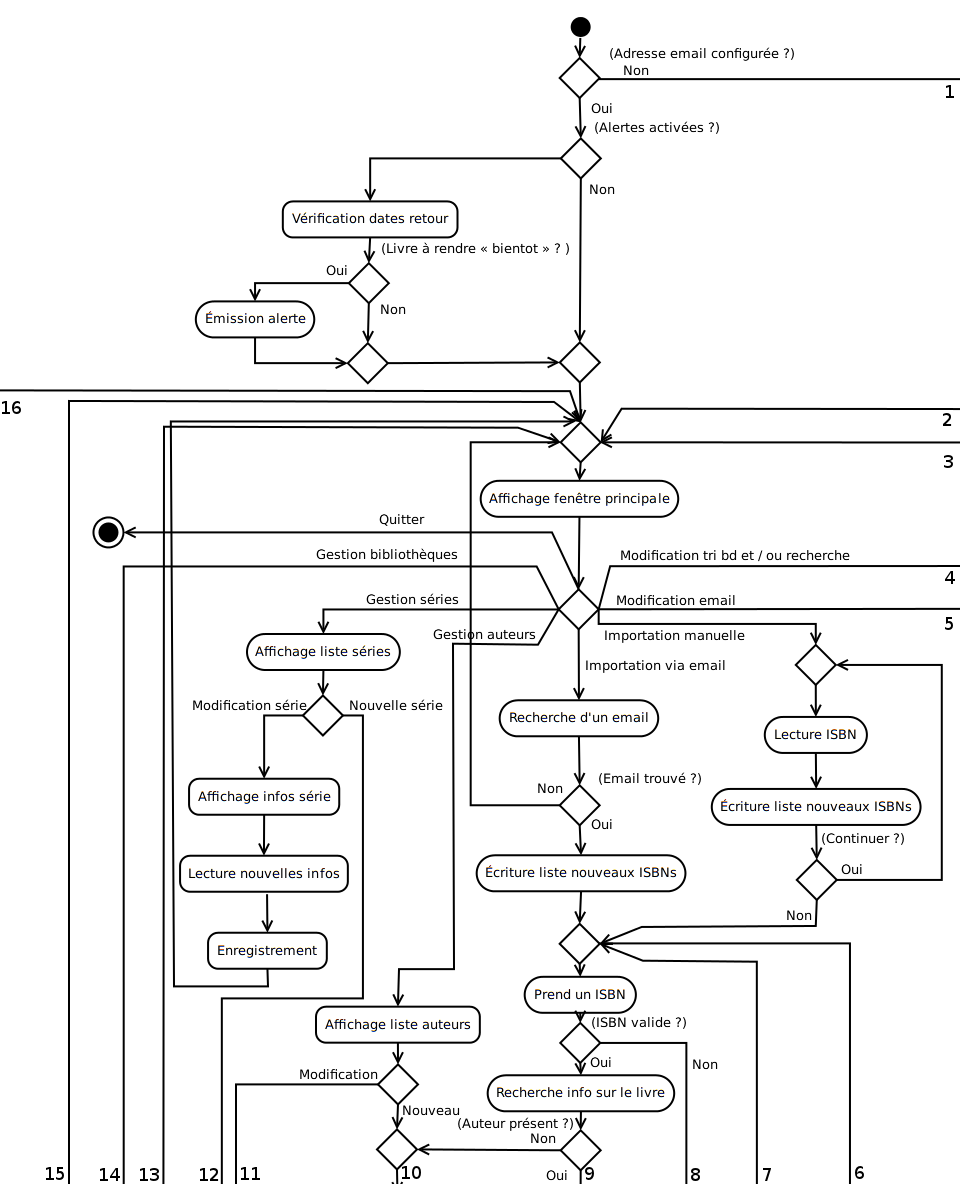
\includegraphics[width=16cm, height=19cm]{uml/appli_pc/p1.png}
\end{center}
\end{figure}
\newpage{} 

\begin{figure}[h!]
\begin{center}
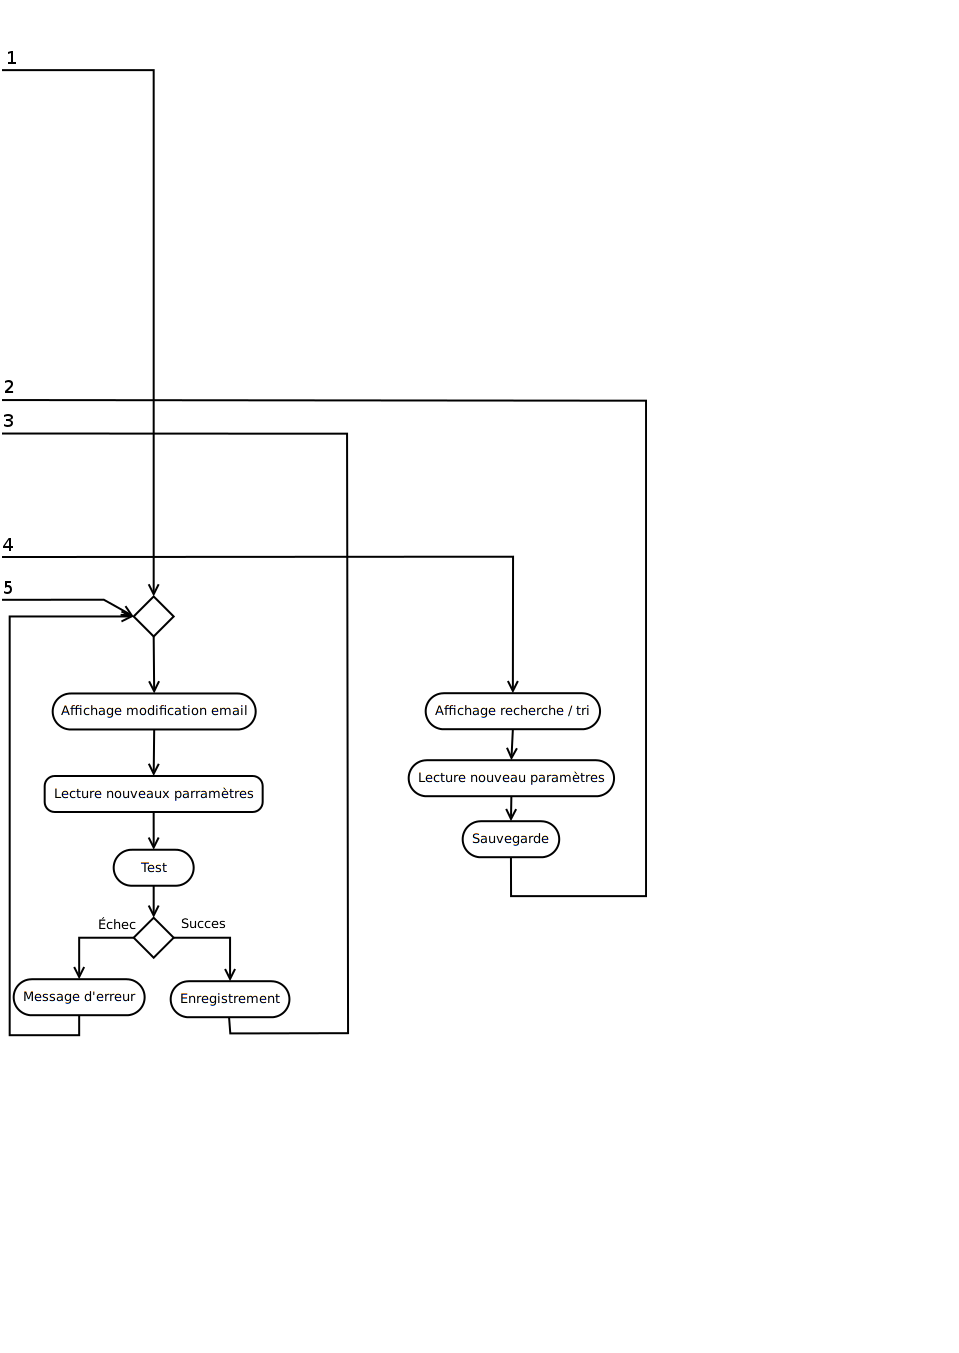
\includegraphics[width=16cm]{uml/appli_pc/p2.png}
\end{center}
\end{figure}
\newpage{}

\begin{figure}[h!]
\begin{center}
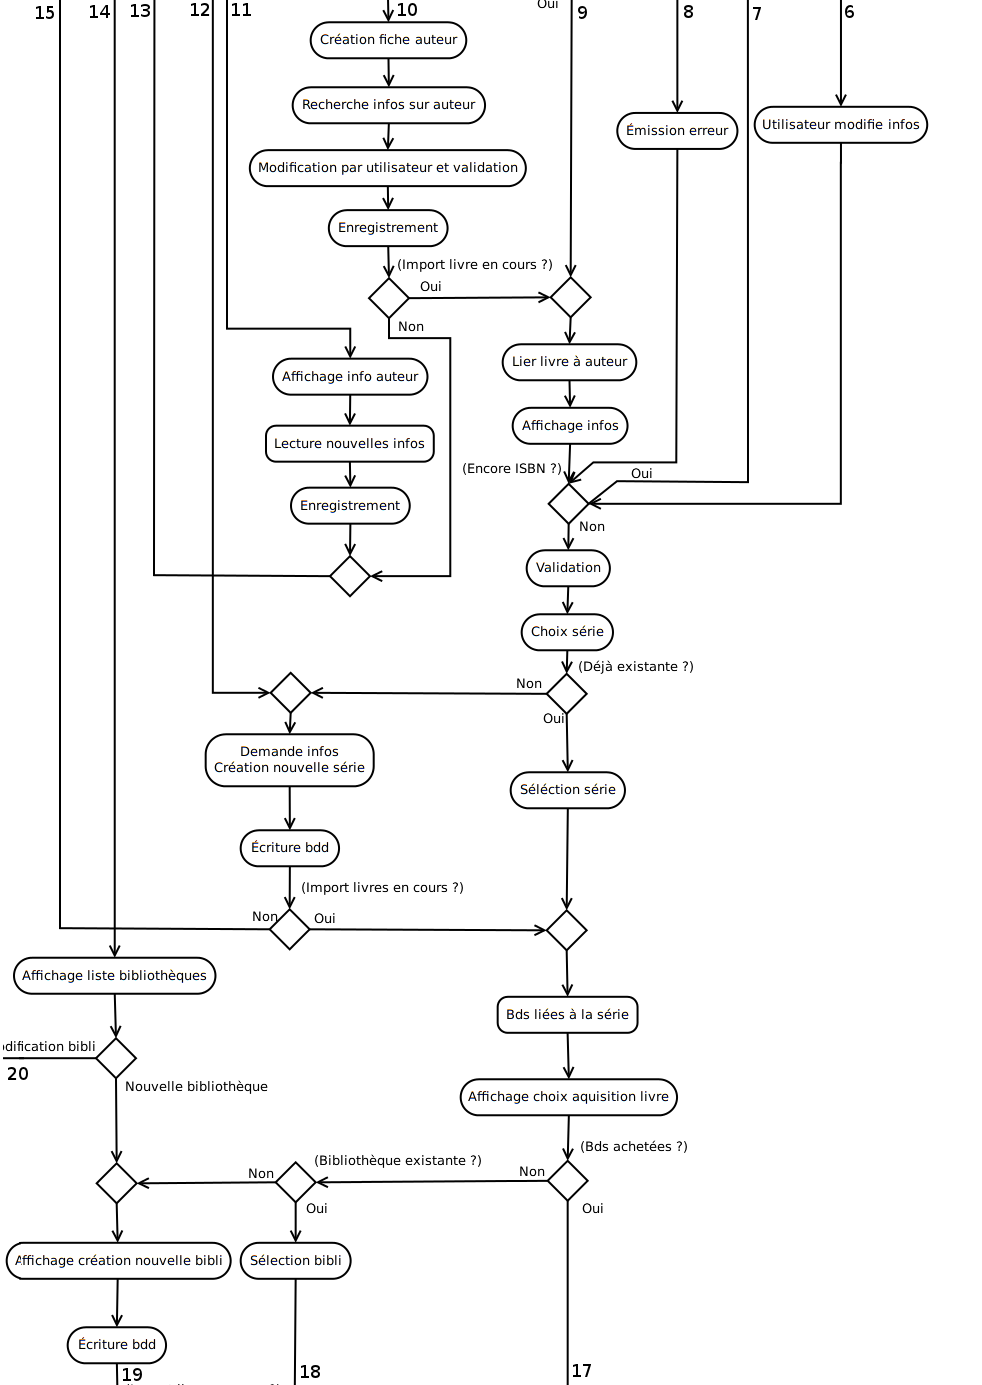
\includegraphics[width=16cm]{uml/appli_pc/p3.png}
\end{center}
\end{figure}
\newpage{}

\begin{figure}[t!]
%\begin{center}
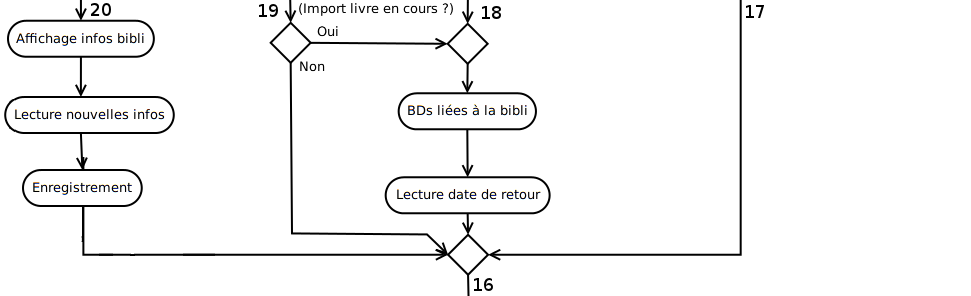
\includegraphics[width=16cm]{uml/appli_pc/p4.png}
%\end{center}
\end{figure}

Tu sais ce que ça veut dire top ou bien ?
